\documentclass[twoside]{book}

% Packages required by doxygen
\usepackage{fixltx2e}
\usepackage{calc}
\usepackage{doxygen}
\usepackage[export]{adjustbox} % also loads graphicx
\usepackage{graphicx}
\usepackage[utf8]{inputenc}
\usepackage{makeidx}
\usepackage{multicol}
\usepackage{multirow}
\PassOptionsToPackage{warn}{textcomp}
\usepackage{textcomp}
\usepackage[nointegrals]{wasysym}
\usepackage[table]{xcolor}

% Font selection
\usepackage[T1]{fontenc}
\usepackage[scaled=.90]{helvet}
\usepackage{courier}
\usepackage{amssymb}
\usepackage{sectsty}
\renewcommand{\familydefault}{\sfdefault}
\allsectionsfont{%
  \fontseries{bc}\selectfont%
  \color{darkgray}%
}
\renewcommand{\DoxyLabelFont}{%
  \fontseries{bc}\selectfont%
  \color{darkgray}%
}
\newcommand{\+}{\discretionary{\mbox{\scriptsize$\hookleftarrow$}}{}{}}

% Page & text layout
\usepackage{geometry}
\geometry{%
  a4paper,%
  top=2.5cm,%
  bottom=2.5cm,%
  left=2.5cm,%
  right=2.5cm%
}
\tolerance=750
\hfuzz=15pt
\hbadness=750
\setlength{\emergencystretch}{15pt}
\setlength{\parindent}{0cm}
\setlength{\parskip}{3ex plus 2ex minus 2ex}
\makeatletter
\renewcommand{\paragraph}{%
  \@startsection{paragraph}{4}{0ex}{-1.0ex}{1.0ex}{%
    \normalfont\normalsize\bfseries\SS@parafont%
  }%
}
\renewcommand{\subparagraph}{%
  \@startsection{subparagraph}{5}{0ex}{-1.0ex}{1.0ex}{%
    \normalfont\normalsize\bfseries\SS@subparafont%
  }%
}
\makeatother

% Headers & footers
\usepackage{fancyhdr}
\pagestyle{fancyplain}
\fancyhead[LE]{\fancyplain{}{\bfseries\thepage}}
\fancyhead[CE]{\fancyplain{}{}}
\fancyhead[RE]{\fancyplain{}{\bfseries\leftmark}}
\fancyhead[LO]{\fancyplain{}{\bfseries\rightmark}}
\fancyhead[CO]{\fancyplain{}{}}
\fancyhead[RO]{\fancyplain{}{\bfseries\thepage}}
\fancyfoot[LE]{\fancyplain{}{}}
\fancyfoot[CE]{\fancyplain{}{}}
\fancyfoot[RE]{\fancyplain{}{\bfseries\scriptsize Generated by Doxygen }}
\fancyfoot[LO]{\fancyplain{}{\bfseries\scriptsize Generated by Doxygen }}
\fancyfoot[CO]{\fancyplain{}{}}
\fancyfoot[RO]{\fancyplain{}{}}
\renewcommand{\footrulewidth}{0.4pt}
\renewcommand{\chaptermark}[1]{%
  \markboth{#1}{}%
}
\renewcommand{\sectionmark}[1]{%
  \markright{\thesection\ #1}%
}

% Indices & bibliography
\usepackage{natbib}
\usepackage[titles]{tocloft}
\setcounter{tocdepth}{3}
\setcounter{secnumdepth}{5}
\makeindex

% Hyperlinks (required, but should be loaded last)
\usepackage{ifpdf}
\ifpdf
  \usepackage[pdftex,pagebackref=true]{hyperref}
\else
  \usepackage[ps2pdf,pagebackref=true]{hyperref}
\fi
\hypersetup{%
  colorlinks=true,%
  linkcolor=blue,%
  citecolor=blue,%
  unicode%
}

% Custom commands
\newcommand{\clearemptydoublepage}{%
  \newpage{\pagestyle{empty}\cleardoublepage}%
}

\usepackage{caption}
\captionsetup{labelsep=space,justification=centering,font={bf},singlelinecheck=off,skip=4pt,position=top}

%===== C O N T E N T S =====

\begin{document}

% Titlepage & ToC
\hypersetup{pageanchor=false,
             bookmarksnumbered=true,
             pdfencoding=unicode
            }
\pagenumbering{alph}
\begin{titlepage}
\vspace*{7cm}
\begin{center}%
{\Large bignum.\+cl }\\
\vspace*{1cm}
{\large Generated by Doxygen 1.8.13}\\
\end{center}
\end{titlepage}
\clearemptydoublepage
\pagenumbering{roman}
\tableofcontents
\clearemptydoublepage
\pagenumbering{arabic}
\hypersetup{pageanchor=true}

%--- Begin generated contents ---
\chapter{Class Index}
\section{Class List}
Here are the classes, structs, unions and interfaces with brief descriptions\+:\begin{DoxyCompactList}
\item\contentsline{section}{\hyperlink{structbignum__t}{bignum\+\_\+t} \\*The type of a big number }{\pageref{structbignum__t}}{}
\end{DoxyCompactList}

\chapter{File Index}
\section{File List}
Here is a list of all files with brief descriptions\+:\begin{DoxyCompactList}
\item\contentsline{section}{src/\hyperlink{bignum_8c}{bignum.\+c} }{\pageref{bignum_8c}}{}
\item\contentsline{section}{src/\hyperlink{bignum_8h}{bignum.\+h} \\*Declares basic types and core functions of the bignum.\+cl library }{\pageref{bignum_8h}}{}
\item\contentsline{section}{tests/\hyperlink{test_8c}{test.\+c} }{\pageref{test_8c}}{}
\item\contentsline{section}{tests/\hyperlink{test__bignum_8c}{test\+\_\+bignum.\+c} \\*Specification of \hyperlink{bignum_8h}{bignum.\+h} }{\pageref{test__bignum_8c}}{}
\end{DoxyCompactList}

\chapter{Class Documentation}
\hypertarget{structbignum}{}\section{bignum Struct Reference}
\label{structbignum}\index{bignum@{bignum}}


The type of a big number.  




{\ttfamily \#include $<$bignum.\+h$>$}

\subsection*{Public Attributes}
\begin{DoxyCompactItemize}
\item 
size\+\_\+t \hyperlink{structbignum_a5cec444ac0a9e7b44a073dbb0f0bf915}{length}
\item 
size\+\_\+t \hyperlink{structbignum_aca95f5f27d2bb952cb8a6f906a138e62}{max\+\_\+length}
\item 
\hyperlink{bignum_8h_a8a2940600ccf96356e2a21b453d3bd92}{bignum\+\_\+elem\+\_\+t} $\ast$ \hyperlink{structbignum_a60955e5f7046ec12c4c292510ad18146}{v}
\end{DoxyCompactItemize}


\subsection{Detailed Description}
The type of a big number. 

More description  None of the members of bignum\+\_\+t should be changed by the user. Doing so can result in undefined behavoir and segmentation faults. 

Definition at line 55 of file bignum.\+h.



\subsection{Member Data Documentation}
\mbox{\Hypertarget{structbignum_a5cec444ac0a9e7b44a073dbb0f0bf915}\label{structbignum_a5cec444ac0a9e7b44a073dbb0f0bf915}} 
\index{bignum@{bignum}!length@{length}}
\index{length@{length}!bignum@{bignum}}
\subsubsection{\texorpdfstring{length}{length}}
{\footnotesize\ttfamily size\+\_\+t bignum\+::length}

The number of elements this bignum actually uses. 

Definition at line 57 of file bignum.\+h.

\mbox{\Hypertarget{structbignum_aca95f5f27d2bb952cb8a6f906a138e62}\label{structbignum_aca95f5f27d2bb952cb8a6f906a138e62}} 
\index{bignum@{bignum}!max\+\_\+length@{max\+\_\+length}}
\index{max\+\_\+length@{max\+\_\+length}!bignum@{bignum}}
\subsubsection{\texorpdfstring{max\+\_\+length}{max\_length}}
{\footnotesize\ttfamily size\+\_\+t bignum\+::max\+\_\+length}

The number of elements this bignum can hold. 

Definition at line 59 of file bignum.\+h.

\mbox{\Hypertarget{structbignum_a60955e5f7046ec12c4c292510ad18146}\label{structbignum_a60955e5f7046ec12c4c292510ad18146}} 
\index{bignum@{bignum}!v@{v}}
\index{v@{v}!bignum@{bignum}}
\subsubsection{\texorpdfstring{v}{v}}
{\footnotesize\ttfamily \hyperlink{bignum_8h_a8a2940600ccf96356e2a21b453d3bd92}{bignum\+\_\+elem\+\_\+t}$\ast$ bignum\+::v}

A pointer to the actual values of this bignum. 

Definition at line 61 of file bignum.\+h.



The documentation for this struct was generated from the following file\+:\begin{DoxyCompactItemize}
\item 
src/\hyperlink{bignum_8h}{bignum.\+h}\end{DoxyCompactItemize}

\chapter{File Documentation}
\hypertarget{bignum_8c}{}\section{src/bignum.c File Reference}
\label{bignum_8c}\index{src/bignum.\+c@{src/bignum.\+c}}
{\ttfamily \#include \char`\"{}bignum.\+h\char`\"{}}\newline
Include dependency graph for bignum.\+c\+:\nopagebreak
\begin{figure}[H]
\begin{center}
\leavevmode
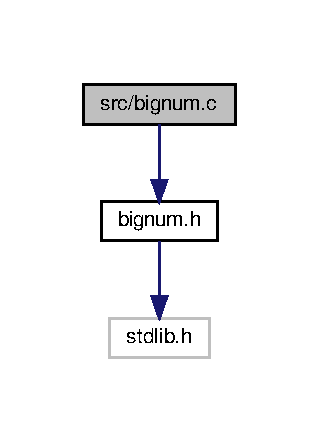
\includegraphics[width=153pt]{bignum_8c__incl}
\end{center}
\end{figure}
\subsection*{Functions}
\begin{DoxyCompactItemize}
\item 
void \hyperlink{bignum_8c_ab18c6d897cc2114df5d05fd6d6e5c3c7}{bignum\+\_\+sync} (\hyperlink{structbignum__t}{bignum\+\_\+t} $\ast$num)
\begin{DoxyCompactList}\small\item\em Synchronize bignum metadata with the underlying memory. \end{DoxyCompactList}\item 
void \hyperlink{bignum_8c_a80f59ecb7ebfd0a18692a21805f7caa2}{bignum\+\_\+assoc} (\hyperlink{structbignum__t}{bignum\+\_\+t} $\ast$num, \hyperlink{bignum_8h_ac19e9b7c8236cb1d9e8b4bf16d0ce513}{bignum\+\_\+elem\+\_\+t} $\ast$arr, const size\+\_\+t num\+\_\+elements)
\begin{DoxyCompactList}\small\item\em Associate num\+\_\+elements in arr with num. \end{DoxyCompactList}\item 
void \hyperlink{bignum_8c_a3b1132294306db3daf600b2a88b341b3}{bignum\+\_\+zero} (\hyperlink{structbignum__t}{bignum\+\_\+t} $\ast$num)
\begin{DoxyCompactList}\small\item\em Zero out all memory associated with num. \end{DoxyCompactList}\item 
int \hyperlink{bignum_8c_ac8664b4358b43e4fed6692dd26f47f13}{bignum\+\_\+set} (\hyperlink{structbignum__t}{bignum\+\_\+t} $\ast$rop, const \hyperlink{structbignum__t}{bignum\+\_\+t} $\ast$op)
\item 
int \hyperlink{bignum_8c_ad9e04b2f22d264e11f8fe35805416929}{bignum\+\_\+set\+\_\+ui} (\hyperlink{structbignum__t}{bignum\+\_\+t} $\ast$rop, const \hyperlink{bignum_8h_ac19e9b7c8236cb1d9e8b4bf16d0ce513}{bignum\+\_\+elem\+\_\+t} op)
\begin{DoxyCompactList}\small\item\em Set rop to the value of op. \end{DoxyCompactList}\item 
int \hyperlink{bignum_8c_aa65b1d0f318d95c53cd9c4ca8a799051}{bignum\+\_\+cmp} (const \hyperlink{structbignum__t}{bignum\+\_\+t} $\ast$op1, const \hyperlink{structbignum__t}{bignum\+\_\+t} $\ast$op2)
\item 
int \hyperlink{bignum_8c_a505aa030e32b81708fa8cceb01ecd600}{bignum\+\_\+cmp\+\_\+ui} (const \hyperlink{structbignum__t}{bignum\+\_\+t} $\ast$op1, const \hyperlink{bignum_8h_ac19e9b7c8236cb1d9e8b4bf16d0ce513}{bignum\+\_\+elem\+\_\+t} op2)
\end{DoxyCompactItemize}


\subsection{Function Documentation}
\mbox{\Hypertarget{bignum_8c_a80f59ecb7ebfd0a18692a21805f7caa2}\label{bignum_8c_a80f59ecb7ebfd0a18692a21805f7caa2}} 
\index{bignum.\+c@{bignum.\+c}!bignum\+\_\+assoc@{bignum\+\_\+assoc}}
\index{bignum\+\_\+assoc@{bignum\+\_\+assoc}!bignum.\+c@{bignum.\+c}}
\subsubsection{\texorpdfstring{bignum\+\_\+assoc()}{bignum\_assoc()}}
{\footnotesize\ttfamily void bignum\+\_\+assoc (\begin{DoxyParamCaption}\item[{\hyperlink{structbignum__t}{bignum\+\_\+t} $\ast$}]{num,  }\item[{\hyperlink{bignum_8h_ac19e9b7c8236cb1d9e8b4bf16d0ce513}{bignum\+\_\+elem\+\_\+t} $\ast$}]{arr,  }\item[{const size\+\_\+t}]{num\+\_\+elements }\end{DoxyParamCaption})}



Associate num\+\_\+elements in arr with num. 

After calling \hyperlink{bignum_8h_a80f59ecb7ebfd0a18692a21805f7caa2}{bignum\+\_\+assoc()} the elements arr\mbox{[}0\mbox{]} to arr\mbox{[}num\+\_\+elements-\/1\mbox{]} will be treated as a big number, which can be accessed through num.

This code will create an array big enough to hold a 1024 bit number and associate the variable x with it\+: 
\begin{DoxyCode}
\hyperlink{structbignum__t}{bignum\_t} x;
\hyperlink{bignum_8h_ac19e9b7c8236cb1d9e8b4bf16d0ce513}{bignum\_elem\_t} x\_elements[\hyperlink{bignum_8h_acff115c908a413aa2479d2883fedec1b}{BIGNUM\_1024}];
\hyperlink{bignum_8c_a80f59ecb7ebfd0a18692a21805f7caa2}{bignum\_assoc}(&x, x\_elements, \hyperlink{bignum_8h_acff115c908a413aa2479d2883fedec1b}{BIGNUM\_1024});
\end{DoxyCode}



\begin{DoxyParams}{Parameters}
{\em num} & The number with which the elements in arr will be associated with. \\
\hline
{\em arr} & The array holding the actual elements. \\
\hline
{\em num\+\_\+elements} & Number of elements from arr to associate with num. \\
\hline
\end{DoxyParams}


Definition at line 17 of file bignum.\+c.

\mbox{\Hypertarget{bignum_8c_aa65b1d0f318d95c53cd9c4ca8a799051}\label{bignum_8c_aa65b1d0f318d95c53cd9c4ca8a799051}} 
\index{bignum.\+c@{bignum.\+c}!bignum\+\_\+cmp@{bignum\+\_\+cmp}}
\index{bignum\+\_\+cmp@{bignum\+\_\+cmp}!bignum.\+c@{bignum.\+c}}
\subsubsection{\texorpdfstring{bignum\+\_\+cmp()}{bignum\_cmp()}}
{\footnotesize\ttfamily int bignum\+\_\+cmp (\begin{DoxyParamCaption}\item[{const \hyperlink{structbignum__t}{bignum\+\_\+t} $\ast$}]{op1,  }\item[{const \hyperlink{structbignum__t}{bignum\+\_\+t} $\ast$}]{op2 }\end{DoxyParamCaption})}

Compare two numbers of type \hyperlink{structbignum__t}{bignum\+\_\+t}

-\/1 if op1 $<$ op2, 1 if op1 $>$ op2 and 0 if both are equal. 

Definition at line 69 of file bignum.\+c.

\mbox{\Hypertarget{bignum_8c_a505aa030e32b81708fa8cceb01ecd600}\label{bignum_8c_a505aa030e32b81708fa8cceb01ecd600}} 
\index{bignum.\+c@{bignum.\+c}!bignum\+\_\+cmp\+\_\+ui@{bignum\+\_\+cmp\+\_\+ui}}
\index{bignum\+\_\+cmp\+\_\+ui@{bignum\+\_\+cmp\+\_\+ui}!bignum.\+c@{bignum.\+c}}
\subsubsection{\texorpdfstring{bignum\+\_\+cmp\+\_\+ui()}{bignum\_cmp\_ui()}}
{\footnotesize\ttfamily int bignum\+\_\+cmp\+\_\+ui (\begin{DoxyParamCaption}\item[{const \hyperlink{structbignum__t}{bignum\+\_\+t} $\ast$}]{op1,  }\item[{const \hyperlink{bignum_8h_ac19e9b7c8236cb1d9e8b4bf16d0ce513}{bignum\+\_\+elem\+\_\+t}}]{op2 }\end{DoxyParamCaption})}

Compare a \hyperlink{structbignum__t}{bignum\+\_\+t} with a bignum\+\_\+elem\+\_\+t.

-\/1 if op1 $<$ op2, 1 if op1 $>$ op2 and 0 if both are equal. 

Definition at line 86 of file bignum.\+c.

\mbox{\Hypertarget{bignum_8c_ac8664b4358b43e4fed6692dd26f47f13}\label{bignum_8c_ac8664b4358b43e4fed6692dd26f47f13}} 
\index{bignum.\+c@{bignum.\+c}!bignum\+\_\+set@{bignum\+\_\+set}}
\index{bignum\+\_\+set@{bignum\+\_\+set}!bignum.\+c@{bignum.\+c}}
\subsubsection{\texorpdfstring{bignum\+\_\+set()}{bignum\_set()}}
{\footnotesize\ttfamily int bignum\+\_\+set (\begin{DoxyParamCaption}\item[{\hyperlink{structbignum__t}{bignum\+\_\+t} $\ast$}]{rop,  }\item[{const \hyperlink{structbignum__t}{bignum\+\_\+t} $\ast$}]{op }\end{DoxyParamCaption})}



Definition at line 36 of file bignum.\+c.

\mbox{\Hypertarget{bignum_8c_ad9e04b2f22d264e11f8fe35805416929}\label{bignum_8c_ad9e04b2f22d264e11f8fe35805416929}} 
\index{bignum.\+c@{bignum.\+c}!bignum\+\_\+set\+\_\+ui@{bignum\+\_\+set\+\_\+ui}}
\index{bignum\+\_\+set\+\_\+ui@{bignum\+\_\+set\+\_\+ui}!bignum.\+c@{bignum.\+c}}
\subsubsection{\texorpdfstring{bignum\+\_\+set\+\_\+ui()}{bignum\_set\_ui()}}
{\footnotesize\ttfamily int bignum\+\_\+set\+\_\+ui (\begin{DoxyParamCaption}\item[{\hyperlink{structbignum__t}{bignum\+\_\+t} $\ast$}]{rop,  }\item[{const \hyperlink{bignum_8h_ac19e9b7c8236cb1d9e8b4bf16d0ce513}{bignum\+\_\+elem\+\_\+t}}]{op }\end{DoxyParamCaption})}



Set rop to the value of op. 



Definition at line 48 of file bignum.\+c.

\mbox{\Hypertarget{bignum_8c_ab18c6d897cc2114df5d05fd6d6e5c3c7}\label{bignum_8c_ab18c6d897cc2114df5d05fd6d6e5c3c7}} 
\index{bignum.\+c@{bignum.\+c}!bignum\+\_\+sync@{bignum\+\_\+sync}}
\index{bignum\+\_\+sync@{bignum\+\_\+sync}!bignum.\+c@{bignum.\+c}}
\subsubsection{\texorpdfstring{bignum\+\_\+sync()}{bignum\_sync()}}
{\footnotesize\ttfamily void bignum\+\_\+sync (\begin{DoxyParamCaption}\item[{\hyperlink{structbignum__t}{bignum\+\_\+t} $\ast$}]{num }\end{DoxyParamCaption})}



Synchronize bignum metadata with the underlying memory. 



Definition at line 9 of file bignum.\+c.

\mbox{\Hypertarget{bignum_8c_a3b1132294306db3daf600b2a88b341b3}\label{bignum_8c_a3b1132294306db3daf600b2a88b341b3}} 
\index{bignum.\+c@{bignum.\+c}!bignum\+\_\+zero@{bignum\+\_\+zero}}
\index{bignum\+\_\+zero@{bignum\+\_\+zero}!bignum.\+c@{bignum.\+c}}
\subsubsection{\texorpdfstring{bignum\+\_\+zero()}{bignum\_zero()}}
{\footnotesize\ttfamily void bignum\+\_\+zero (\begin{DoxyParamCaption}\item[{\hyperlink{structbignum__t}{bignum\+\_\+t} $\ast$}]{num }\end{DoxyParamCaption})}



Zero out all memory associated with num. 



Definition at line 24 of file bignum.\+c.


\hypertarget{bignum_8h}{}\section{src/bignum.h File Reference}
\label{bignum_8h}\index{src/bignum.\+h@{src/bignum.\+h}}


Declares basic types and core functions of the bignum.\+cl library.  


{\ttfamily \#include $<$stdlib.\+h$>$}\newline
Include dependency graph for bignum.\+h\+:\nopagebreak
\begin{figure}[H]
\begin{center}
\leavevmode
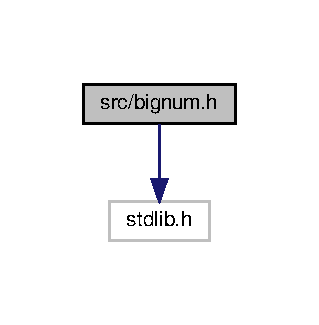
\includegraphics[width=153pt]{bignum_8h__incl}
\end{center}
\end{figure}
This graph shows which files directly or indirectly include this file\+:
\nopagebreak
\begin{figure}[H]
\begin{center}
\leavevmode
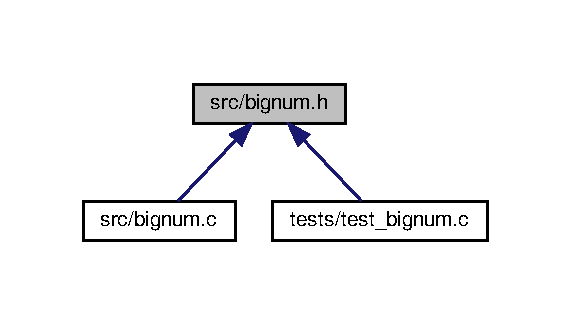
\includegraphics[width=274pt]{bignum_8h__dep__incl}
\end{center}
\end{figure}
\subsection*{Classes}
\begin{DoxyCompactItemize}
\item 
struct \hyperlink{structbignum__t}{bignum\+\_\+t}
\begin{DoxyCompactList}\small\item\em The type of a big number. \end{DoxyCompactList}\end{DoxyCompactItemize}
\subsection*{Macros}
\begin{DoxyCompactItemize}
\item 
\#define \hyperlink{bignum_8h_aae679f6820f99b2e064916c3594c582a}{B\+I\+G\+N\+U\+M\+\_\+\+T\+Y\+PE}~unsigned long
\begin{DoxyCompactList}\small\item\em Defines the datatype used by bignum\+\_\+elem\+\_\+t. \end{DoxyCompactList}\item 
\#define \hyperlink{bignum_8h_adc0dc33688c900c97fa94c7a795554b1}{B\+I\+G\+N\+U\+M\+\_\+512}~(64 / sizeof(\hyperlink{bignum_8h_ac19e9b7c8236cb1d9e8b4bf16d0ce513}{bignum\+\_\+elem\+\_\+t}))
\begin{DoxyCompactList}\small\item\em array size required for 512 bit numbers \end{DoxyCompactList}\item 
\#define \hyperlink{bignum_8h_acff115c908a413aa2479d2883fedec1b}{B\+I\+G\+N\+U\+M\+\_\+1024}~(\hyperlink{bignum_8h_adc0dc33688c900c97fa94c7a795554b1}{B\+I\+G\+N\+U\+M\+\_\+512}$\ast$2)
\begin{DoxyCompactList}\small\item\em array size required for 1024 bit numbers \end{DoxyCompactList}\item 
\#define \hyperlink{bignum_8h_ae53df04bbf79c53f0f5bb23ae6a3f198}{B\+I\+G\+N\+U\+M\+\_\+2048}~(\hyperlink{bignum_8h_adc0dc33688c900c97fa94c7a795554b1}{B\+I\+G\+N\+U\+M\+\_\+512}$\ast$4)
\begin{DoxyCompactList}\small\item\em array size required for 2048 bit numbers \end{DoxyCompactList}\item 
\#define \hyperlink{bignum_8h_a59d692e5e6488e51a82e6f8ec7183575}{B\+I\+G\+N\+U\+M\+\_\+4096}~(\hyperlink{bignum_8h_adc0dc33688c900c97fa94c7a795554b1}{B\+I\+G\+N\+U\+M\+\_\+512}$\ast$8)
\begin{DoxyCompactList}\small\item\em array size required for 4096 bit numbers \end{DoxyCompactList}\end{DoxyCompactItemize}
\subsection*{Typedefs}
\begin{DoxyCompactItemize}
\item 
typedef \hyperlink{bignum_8h_aae679f6820f99b2e064916c3594c582a}{B\+I\+G\+N\+U\+M\+\_\+\+T\+Y\+PE} \hyperlink{bignum_8h_ac19e9b7c8236cb1d9e8b4bf16d0ce513}{bignum\+\_\+elem\+\_\+t}
\begin{DoxyCompactList}\small\item\em The type of the elements of a big number. \end{DoxyCompactList}\end{DoxyCompactItemize}
\subsection*{Functions}
\begin{DoxyCompactItemize}
\item 
void \hyperlink{bignum_8h_a80f59ecb7ebfd0a18692a21805f7caa2}{bignum\+\_\+assoc} (\hyperlink{structbignum__t}{bignum\+\_\+t} $\ast$num, \hyperlink{bignum_8h_ac19e9b7c8236cb1d9e8b4bf16d0ce513}{bignum\+\_\+elem\+\_\+t} $\ast$arr, const size\+\_\+t num\+\_\+elements)
\begin{DoxyCompactList}\small\item\em Associate num\+\_\+elements in arr with num. \end{DoxyCompactList}\item 
void \hyperlink{bignum_8h_ab18c6d897cc2114df5d05fd6d6e5c3c7}{bignum\+\_\+sync} (\hyperlink{structbignum__t}{bignum\+\_\+t} $\ast$num)
\begin{DoxyCompactList}\small\item\em Synchronize bignum metadata with the underlying memory. \end{DoxyCompactList}\item 
void \hyperlink{bignum_8h_a3b1132294306db3daf600b2a88b341b3}{bignum\+\_\+zero} (\hyperlink{structbignum__t}{bignum\+\_\+t} $\ast$num)
\begin{DoxyCompactList}\small\item\em Zero out all memory associated with num. \end{DoxyCompactList}\item 
int \hyperlink{bignum_8h_ac8664b4358b43e4fed6692dd26f47f13}{bignum\+\_\+set} (\hyperlink{structbignum__t}{bignum\+\_\+t} $\ast$rop, const \hyperlink{structbignum__t}{bignum\+\_\+t} $\ast$op)
\item 
int \hyperlink{bignum_8h_ad9e04b2f22d264e11f8fe35805416929}{bignum\+\_\+set\+\_\+ui} (\hyperlink{structbignum__t}{bignum\+\_\+t} $\ast$rop, const \hyperlink{bignum_8h_ac19e9b7c8236cb1d9e8b4bf16d0ce513}{bignum\+\_\+elem\+\_\+t} op)
\begin{DoxyCompactList}\small\item\em Set rop to the value of op. \end{DoxyCompactList}\item 
int \hyperlink{bignum_8h_aa65b1d0f318d95c53cd9c4ca8a799051}{bignum\+\_\+cmp} (const \hyperlink{structbignum__t}{bignum\+\_\+t} $\ast$op1, const \hyperlink{structbignum__t}{bignum\+\_\+t} $\ast$op2)
\item 
int \hyperlink{bignum_8h_a505aa030e32b81708fa8cceb01ecd600}{bignum\+\_\+cmp\+\_\+ui} (const \hyperlink{structbignum__t}{bignum\+\_\+t} $\ast$op1, const \hyperlink{bignum_8h_ac19e9b7c8236cb1d9e8b4bf16d0ce513}{bignum\+\_\+elem\+\_\+t} op2)
\end{DoxyCompactItemize}


\subsection{Detailed Description}
Declares basic types and core functions of the bignum.\+cl library. 

\subsection*{Memory association}

A core principle of the bignum.\+cl library is memory association. 

\subsection{Macro Definition Documentation}
\mbox{\Hypertarget{bignum_8h_acff115c908a413aa2479d2883fedec1b}\label{bignum_8h_acff115c908a413aa2479d2883fedec1b}} 
\index{bignum.\+h@{bignum.\+h}!B\+I\+G\+N\+U\+M\+\_\+1024@{B\+I\+G\+N\+U\+M\+\_\+1024}}
\index{B\+I\+G\+N\+U\+M\+\_\+1024@{B\+I\+G\+N\+U\+M\+\_\+1024}!bignum.\+h@{bignum.\+h}}
\subsubsection{\texorpdfstring{B\+I\+G\+N\+U\+M\+\_\+1024}{BIGNUM\_1024}}
{\footnotesize\ttfamily \#define B\+I\+G\+N\+U\+M\+\_\+1024~(\hyperlink{bignum_8h_adc0dc33688c900c97fa94c7a795554b1}{B\+I\+G\+N\+U\+M\+\_\+512}$\ast$2)}



array size required for 1024 bit numbers 



Definition at line 67 of file bignum.\+h.

\mbox{\Hypertarget{bignum_8h_ae53df04bbf79c53f0f5bb23ae6a3f198}\label{bignum_8h_ae53df04bbf79c53f0f5bb23ae6a3f198}} 
\index{bignum.\+h@{bignum.\+h}!B\+I\+G\+N\+U\+M\+\_\+2048@{B\+I\+G\+N\+U\+M\+\_\+2048}}
\index{B\+I\+G\+N\+U\+M\+\_\+2048@{B\+I\+G\+N\+U\+M\+\_\+2048}!bignum.\+h@{bignum.\+h}}
\subsubsection{\texorpdfstring{B\+I\+G\+N\+U\+M\+\_\+2048}{BIGNUM\_2048}}
{\footnotesize\ttfamily \#define B\+I\+G\+N\+U\+M\+\_\+2048~(\hyperlink{bignum_8h_adc0dc33688c900c97fa94c7a795554b1}{B\+I\+G\+N\+U\+M\+\_\+512}$\ast$4)}



array size required for 2048 bit numbers 



Definition at line 69 of file bignum.\+h.

\mbox{\Hypertarget{bignum_8h_a59d692e5e6488e51a82e6f8ec7183575}\label{bignum_8h_a59d692e5e6488e51a82e6f8ec7183575}} 
\index{bignum.\+h@{bignum.\+h}!B\+I\+G\+N\+U\+M\+\_\+4096@{B\+I\+G\+N\+U\+M\+\_\+4096}}
\index{B\+I\+G\+N\+U\+M\+\_\+4096@{B\+I\+G\+N\+U\+M\+\_\+4096}!bignum.\+h@{bignum.\+h}}
\subsubsection{\texorpdfstring{B\+I\+G\+N\+U\+M\+\_\+4096}{BIGNUM\_4096}}
{\footnotesize\ttfamily \#define B\+I\+G\+N\+U\+M\+\_\+4096~(\hyperlink{bignum_8h_adc0dc33688c900c97fa94c7a795554b1}{B\+I\+G\+N\+U\+M\+\_\+512}$\ast$8)}



array size required for 4096 bit numbers 



Definition at line 71 of file bignum.\+h.

\mbox{\Hypertarget{bignum_8h_adc0dc33688c900c97fa94c7a795554b1}\label{bignum_8h_adc0dc33688c900c97fa94c7a795554b1}} 
\index{bignum.\+h@{bignum.\+h}!B\+I\+G\+N\+U\+M\+\_\+512@{B\+I\+G\+N\+U\+M\+\_\+512}}
\index{B\+I\+G\+N\+U\+M\+\_\+512@{B\+I\+G\+N\+U\+M\+\_\+512}!bignum.\+h@{bignum.\+h}}
\subsubsection{\texorpdfstring{B\+I\+G\+N\+U\+M\+\_\+512}{BIGNUM\_512}}
{\footnotesize\ttfamily \#define B\+I\+G\+N\+U\+M\+\_\+512~(64 / sizeof(\hyperlink{bignum_8h_ac19e9b7c8236cb1d9e8b4bf16d0ce513}{bignum\+\_\+elem\+\_\+t}))}



array size required for 512 bit numbers 



Definition at line 65 of file bignum.\+h.

\mbox{\Hypertarget{bignum_8h_aae679f6820f99b2e064916c3594c582a}\label{bignum_8h_aae679f6820f99b2e064916c3594c582a}} 
\index{bignum.\+h@{bignum.\+h}!B\+I\+G\+N\+U\+M\+\_\+\+T\+Y\+PE@{B\+I\+G\+N\+U\+M\+\_\+\+T\+Y\+PE}}
\index{B\+I\+G\+N\+U\+M\+\_\+\+T\+Y\+PE@{B\+I\+G\+N\+U\+M\+\_\+\+T\+Y\+PE}!bignum.\+h@{bignum.\+h}}
\subsubsection{\texorpdfstring{B\+I\+G\+N\+U\+M\+\_\+\+T\+Y\+PE}{BIGNUM\_TYPE}}
{\footnotesize\ttfamily \#define B\+I\+G\+N\+U\+M\+\_\+\+T\+Y\+PE~unsigned long}



Defines the datatype used by bignum\+\_\+elem\+\_\+t. 

You can change the default value by defining B\+I\+G\+N\+U\+M\+\_\+\+T\+Y\+PE yourself. The makros B\+I\+G\+N\+U\+M\+\_\+512, etc. will be working regardless of the underlying bignum\+\_\+elem\+\_\+t datatype\+:

With 32bit unsigned ints this code will set B\+I\+G\+N\+U\+M\+\_\+512 to 16. 
\begin{DoxyCode}
\textcolor{preprocessor}{#define BIGNUM\_TYPE unsigned int}
\textcolor{preprocessor}{#include "bignum.h"}
\end{DoxyCode}


With 8 bit unsigned chars this code will set B\+I\+G\+N\+U\+M\+\_\+512 to 64. 
\begin{DoxyCode}
\textcolor{preprocessor}{#define BIGNUM\_TYPE unsigned char}
\textcolor{preprocessor}{#include "bignum.h"}
\end{DoxyCode}


In both cases the maximum value represented by a \hyperlink{structbignum__t}{bignum\+\_\+t} used with B\+I\+G\+N\+U\+M\+\_\+512 will be 2$^\wedge$512 -\/ 1.

\begin{DoxyWarning}{Warning}
Setting B\+I\+G\+N\+U\+M\+\_\+\+T\+Y\+PE to a signed datatype will result in undefined behavoir. 
\end{DoxyWarning}


Definition at line 42 of file bignum.\+h.



\subsection{Typedef Documentation}
\mbox{\Hypertarget{bignum_8h_ac19e9b7c8236cb1d9e8b4bf16d0ce513}\label{bignum_8h_ac19e9b7c8236cb1d9e8b4bf16d0ce513}} 
\index{bignum.\+h@{bignum.\+h}!bignum\+\_\+elem\+\_\+t@{bignum\+\_\+elem\+\_\+t}}
\index{bignum\+\_\+elem\+\_\+t@{bignum\+\_\+elem\+\_\+t}!bignum.\+h@{bignum.\+h}}
\subsubsection{\texorpdfstring{bignum\+\_\+elem\+\_\+t}{bignum\_elem\_t}}
{\footnotesize\ttfamily typedef \hyperlink{bignum_8h_aae679f6820f99b2e064916c3594c582a}{B\+I\+G\+N\+U\+M\+\_\+\+T\+Y\+PE} \hyperlink{bignum_8h_ac19e9b7c8236cb1d9e8b4bf16d0ce513}{bignum\+\_\+elem\+\_\+t}}



The type of the elements of a big number. 



Definition at line 46 of file bignum.\+h.



\subsection{Function Documentation}
\mbox{\Hypertarget{bignum_8h_a80f59ecb7ebfd0a18692a21805f7caa2}\label{bignum_8h_a80f59ecb7ebfd0a18692a21805f7caa2}} 
\index{bignum.\+h@{bignum.\+h}!bignum\+\_\+assoc@{bignum\+\_\+assoc}}
\index{bignum\+\_\+assoc@{bignum\+\_\+assoc}!bignum.\+h@{bignum.\+h}}
\subsubsection{\texorpdfstring{bignum\+\_\+assoc()}{bignum\_assoc()}}
{\footnotesize\ttfamily void bignum\+\_\+assoc (\begin{DoxyParamCaption}\item[{\hyperlink{structbignum__t}{bignum\+\_\+t} $\ast$}]{num,  }\item[{\hyperlink{bignum_8h_ac19e9b7c8236cb1d9e8b4bf16d0ce513}{bignum\+\_\+elem\+\_\+t} $\ast$}]{arr,  }\item[{const size\+\_\+t}]{num\+\_\+elements }\end{DoxyParamCaption})}



Associate num\+\_\+elements in arr with num. 

After calling \hyperlink{bignum_8h_a80f59ecb7ebfd0a18692a21805f7caa2}{bignum\+\_\+assoc()} the elements arr\mbox{[}0\mbox{]} to arr\mbox{[}num\+\_\+elements-\/1\mbox{]} will be treated as a big number, which can be accessed through num.

This code will create an array big enough to hold a 1024 bit number and associate the variable x with it\+: 
\begin{DoxyCode}
\hyperlink{structbignum__t}{bignum\_t} x;
\hyperlink{bignum_8h_ac19e9b7c8236cb1d9e8b4bf16d0ce513}{bignum\_elem\_t} x\_elements[\hyperlink{bignum_8h_acff115c908a413aa2479d2883fedec1b}{BIGNUM\_1024}];
\hyperlink{bignum_8c_a80f59ecb7ebfd0a18692a21805f7caa2}{bignum\_assoc}(&x, x\_elements, \hyperlink{bignum_8h_acff115c908a413aa2479d2883fedec1b}{BIGNUM\_1024});
\end{DoxyCode}



\begin{DoxyParams}{Parameters}
{\em num} & The number with which the elements in arr will be associated with. \\
\hline
{\em arr} & The array holding the actual elements. \\
\hline
{\em num\+\_\+elements} & Number of elements from arr to associate with num. \\
\hline
\end{DoxyParams}


Definition at line 17 of file bignum.\+c.

\mbox{\Hypertarget{bignum_8h_aa65b1d0f318d95c53cd9c4ca8a799051}\label{bignum_8h_aa65b1d0f318d95c53cd9c4ca8a799051}} 
\index{bignum.\+h@{bignum.\+h}!bignum\+\_\+cmp@{bignum\+\_\+cmp}}
\index{bignum\+\_\+cmp@{bignum\+\_\+cmp}!bignum.\+h@{bignum.\+h}}
\subsubsection{\texorpdfstring{bignum\+\_\+cmp()}{bignum\_cmp()}}
{\footnotesize\ttfamily int bignum\+\_\+cmp (\begin{DoxyParamCaption}\item[{const \hyperlink{structbignum__t}{bignum\+\_\+t} $\ast$}]{op1,  }\item[{const \hyperlink{structbignum__t}{bignum\+\_\+t} $\ast$}]{op2 }\end{DoxyParamCaption})}

Compare two numbers of type \hyperlink{structbignum__t}{bignum\+\_\+t}

-\/1 if op1 $<$ op2, 1 if op1 $>$ op2 and 0 if both are equal. 

Definition at line 69 of file bignum.\+c.

\mbox{\Hypertarget{bignum_8h_a505aa030e32b81708fa8cceb01ecd600}\label{bignum_8h_a505aa030e32b81708fa8cceb01ecd600}} 
\index{bignum.\+h@{bignum.\+h}!bignum\+\_\+cmp\+\_\+ui@{bignum\+\_\+cmp\+\_\+ui}}
\index{bignum\+\_\+cmp\+\_\+ui@{bignum\+\_\+cmp\+\_\+ui}!bignum.\+h@{bignum.\+h}}
\subsubsection{\texorpdfstring{bignum\+\_\+cmp\+\_\+ui()}{bignum\_cmp\_ui()}}
{\footnotesize\ttfamily int bignum\+\_\+cmp\+\_\+ui (\begin{DoxyParamCaption}\item[{const \hyperlink{structbignum__t}{bignum\+\_\+t} $\ast$}]{op1,  }\item[{const \hyperlink{bignum_8h_ac19e9b7c8236cb1d9e8b4bf16d0ce513}{bignum\+\_\+elem\+\_\+t}}]{op2 }\end{DoxyParamCaption})}

Compare a \hyperlink{structbignum__t}{bignum\+\_\+t} with a bignum\+\_\+elem\+\_\+t.

-\/1 if op1 $<$ op2, 1 if op1 $>$ op2 and 0 if both are equal. 

Definition at line 86 of file bignum.\+c.

\mbox{\Hypertarget{bignum_8h_ac8664b4358b43e4fed6692dd26f47f13}\label{bignum_8h_ac8664b4358b43e4fed6692dd26f47f13}} 
\index{bignum.\+h@{bignum.\+h}!bignum\+\_\+set@{bignum\+\_\+set}}
\index{bignum\+\_\+set@{bignum\+\_\+set}!bignum.\+h@{bignum.\+h}}
\subsubsection{\texorpdfstring{bignum\+\_\+set()}{bignum\_set()}}
{\footnotesize\ttfamily int bignum\+\_\+set (\begin{DoxyParamCaption}\item[{\hyperlink{structbignum__t}{bignum\+\_\+t} $\ast$}]{rop,  }\item[{const \hyperlink{structbignum__t}{bignum\+\_\+t} $\ast$}]{op }\end{DoxyParamCaption})}



Definition at line 36 of file bignum.\+c.

\mbox{\Hypertarget{bignum_8h_ad9e04b2f22d264e11f8fe35805416929}\label{bignum_8h_ad9e04b2f22d264e11f8fe35805416929}} 
\index{bignum.\+h@{bignum.\+h}!bignum\+\_\+set\+\_\+ui@{bignum\+\_\+set\+\_\+ui}}
\index{bignum\+\_\+set\+\_\+ui@{bignum\+\_\+set\+\_\+ui}!bignum.\+h@{bignum.\+h}}
\subsubsection{\texorpdfstring{bignum\+\_\+set\+\_\+ui()}{bignum\_set\_ui()}}
{\footnotesize\ttfamily int bignum\+\_\+set\+\_\+ui (\begin{DoxyParamCaption}\item[{\hyperlink{structbignum__t}{bignum\+\_\+t} $\ast$}]{rop,  }\item[{const \hyperlink{bignum_8h_ac19e9b7c8236cb1d9e8b4bf16d0ce513}{bignum\+\_\+elem\+\_\+t}}]{op }\end{DoxyParamCaption})}



Set rop to the value of op. 



Definition at line 48 of file bignum.\+c.

\mbox{\Hypertarget{bignum_8h_ab18c6d897cc2114df5d05fd6d6e5c3c7}\label{bignum_8h_ab18c6d897cc2114df5d05fd6d6e5c3c7}} 
\index{bignum.\+h@{bignum.\+h}!bignum\+\_\+sync@{bignum\+\_\+sync}}
\index{bignum\+\_\+sync@{bignum\+\_\+sync}!bignum.\+h@{bignum.\+h}}
\subsubsection{\texorpdfstring{bignum\+\_\+sync()}{bignum\_sync()}}
{\footnotesize\ttfamily void bignum\+\_\+sync (\begin{DoxyParamCaption}\item[{\hyperlink{structbignum__t}{bignum\+\_\+t} $\ast$}]{num }\end{DoxyParamCaption})}



Synchronize bignum metadata with the underlying memory. 



Definition at line 9 of file bignum.\+c.

\mbox{\Hypertarget{bignum_8h_a3b1132294306db3daf600b2a88b341b3}\label{bignum_8h_a3b1132294306db3daf600b2a88b341b3}} 
\index{bignum.\+h@{bignum.\+h}!bignum\+\_\+zero@{bignum\+\_\+zero}}
\index{bignum\+\_\+zero@{bignum\+\_\+zero}!bignum.\+h@{bignum.\+h}}
\subsubsection{\texorpdfstring{bignum\+\_\+zero()}{bignum\_zero()}}
{\footnotesize\ttfamily void bignum\+\_\+zero (\begin{DoxyParamCaption}\item[{\hyperlink{structbignum__t}{bignum\+\_\+t} $\ast$}]{num }\end{DoxyParamCaption})}



Zero out all memory associated with num. 



Definition at line 24 of file bignum.\+c.


\hypertarget{test_8c}{}\section{tests/test.c File Reference}
\label{test_8c}\index{tests/test.\+c@{tests/test.\+c}}
{\ttfamily \#include $<$stdio.\+h$>$}\newline
Include dependency graph for test.\+c\+:
\nopagebreak
\begin{figure}[H]
\begin{center}
\leavevmode
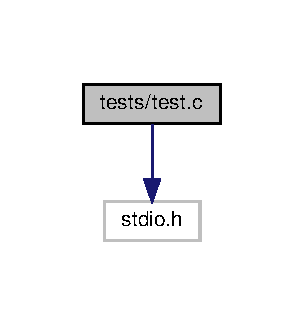
\includegraphics[width=146pt]{test_8c__incl}
\end{center}
\end{figure}
This graph shows which files directly or indirectly include this file\+:
\nopagebreak
\begin{figure}[H]
\begin{center}
\leavevmode
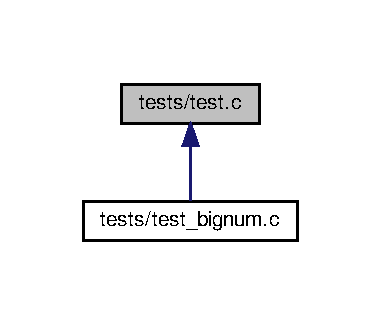
\includegraphics[width=183pt]{test_8c__dep__incl}
\end{center}
\end{figure}
\subsection*{Functions}
\begin{DoxyCompactItemize}
\item 
void \hyperlink{test_8c_a6bc02d5b667ea1f699c919a4b4c4c381}{run\+\_\+test} (char $\ast$desc, int($\ast$test)())
\end{DoxyCompactItemize}
\subsection*{Variables}
\begin{DoxyCompactItemize}
\item 
int \hyperlink{test_8c_af1d037d93bcddd9a8424522dea921a98}{test\+\_\+status} = 0
\end{DoxyCompactItemize}


\subsection{Function Documentation}
\mbox{\Hypertarget{test_8c_a6bc02d5b667ea1f699c919a4b4c4c381}\label{test_8c_a6bc02d5b667ea1f699c919a4b4c4c381}} 
\index{test.\+c@{test.\+c}!run\+\_\+test@{run\+\_\+test}}
\index{run\+\_\+test@{run\+\_\+test}!test.\+c@{test.\+c}}
\subsubsection{\texorpdfstring{run\+\_\+test()}{run\_test()}}
{\footnotesize\ttfamily void run\+\_\+test (\begin{DoxyParamCaption}\item[{char $\ast$}]{desc,  }\item[{int($\ast$)()}]{test }\end{DoxyParamCaption})}



Definition at line 5 of file test.\+c.



\subsection{Variable Documentation}
\mbox{\Hypertarget{test_8c_af1d037d93bcddd9a8424522dea921a98}\label{test_8c_af1d037d93bcddd9a8424522dea921a98}} 
\index{test.\+c@{test.\+c}!test\+\_\+status@{test\+\_\+status}}
\index{test\+\_\+status@{test\+\_\+status}!test.\+c@{test.\+c}}
\subsubsection{\texorpdfstring{test\+\_\+status}{test\_status}}
{\footnotesize\ttfamily int test\+\_\+status = 0}



Definition at line 3 of file test.\+c.


\hypertarget{test__bignum_8c}{}\section{tests/test\+\_\+bignum.c File Reference}
\label{test__bignum_8c}\index{tests/test\+\_\+bignum.\+c@{tests/test\+\_\+bignum.\+c}}


Specification of \hyperlink{bignum_8h}{bignum.\+h}.  


{\ttfamily \#include $<$stdio.\+h$>$}\newline
{\ttfamily \#include \char`\"{}bignum.\+h\char`\"{}}\newline
{\ttfamily \#include \char`\"{}test.\+c\char`\"{}}\newline
Include dependency graph for test\+\_\+bignum.\+c\+:
\nopagebreak
\begin{figure}[H]
\begin{center}
\leavevmode
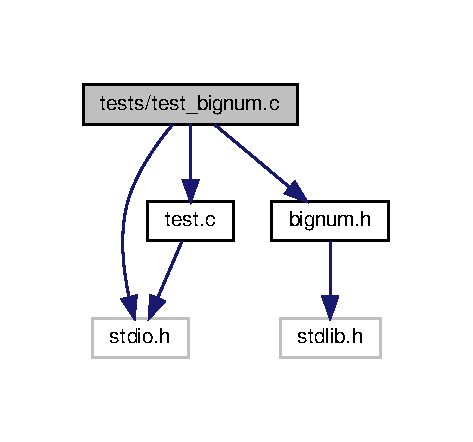
\includegraphics[width=227pt]{test__bignum_8c__incl}
\end{center}
\end{figure}
\subsection*{Functions}
\begin{DoxyCompactItemize}
\item 
int \hyperlink{test__bignum_8c_a0294d67cb325c5bbf965caae1fd5b60e}{test\+\_\+assoc\+\_\+max\+\_\+length} ()
\begin{DoxyCompactList}\small\item\em Associating a \hyperlink{structbignum__t}{bignum\+\_\+t} number with n elements of an array sets the max\+\_\+length metadata to n. \end{DoxyCompactList}\item 
int \hyperlink{test__bignum_8c_a3cb26d281b5fd65f719e2868ae098c96}{test\+\_\+assoc\+\_\+length} ()
\begin{DoxyCompactList}\small\item\em Associating a \hyperlink{structbignum__t}{bignum\+\_\+t} number with an array with exact n nonzero lower elements sets the length metadata to n. \end{DoxyCompactList}\item 
int \hyperlink{test__bignum_8c_a098327c2f0d8b8471d0a3a1439684419}{test\+\_\+assoc\+\_\+zero\+\_\+null} ()
\begin{DoxyCompactList}\small\item\em Associating a \hyperlink{structbignum__t}{bignum\+\_\+t} number with 0 elements of N\+U\+LL, sets the length and max\+\_\+length metadata to 0 and does not cause any errors. \end{DoxyCompactList}\item 
int \hyperlink{test__bignum_8c_ace02da2369ccb38d5aa6103305b7c987}{test\+\_\+assoc\+\_\+zero} ()
\begin{DoxyCompactList}\small\item\em Associating a \hyperlink{structbignum__t}{bignum\+\_\+t} number with 0 elements of an array sets the length and max\+\_\+length metadata to 0 and does not cause any errors. \end{DoxyCompactList}\item 
int \hyperlink{test__bignum_8c_a8d6dfd8cca8c52cc57a0f21d7342b8b9}{test\+\_\+sync\+\_\+length} ()
\begin{DoxyCompactList}\small\item\em Calling bignum\+\_\+sync sets the correct length on a \hyperlink{structbignum__t}{bignum\+\_\+t}. \end{DoxyCompactList}\item 
int \hyperlink{test__bignum_8c_a3c5186feb294d19dcb03ea02123854d1}{test\+\_\+zero\+\_\+data} ()
\begin{DoxyCompactList}\small\item\em Calling \hyperlink{bignum_8c_a3b1132294306db3daf600b2a88b341b3}{bignum\+\_\+zero()} will zero out all associated data and nothing more. \end{DoxyCompactList}\item 
int \hyperlink{test__bignum_8c_a905b4a3ad625c43e956042f64e2f5b10}{test\+\_\+zero\+\_\+data\+\_\+wrong\+\_\+length} ()
\begin{DoxyCompactList}\small\item\em Calling \hyperlink{bignum_8c_a3b1132294306db3daf600b2a88b341b3}{bignum\+\_\+zero()} will zero out all associated data and nothing more, even if the length member of the \hyperlink{structbignum__t}{bignum\+\_\+t} doesn\textquotesingle{}t match with the associated data. \end{DoxyCompactList}\item 
int \hyperlink{test__bignum_8c_ae4202f9280c805042edd0e06d8474220}{test\+\_\+zero\+\_\+length} ()
\begin{DoxyCompactList}\small\item\em Calling \hyperlink{bignum_8c_a3b1132294306db3daf600b2a88b341b3}{bignum\+\_\+zero()} will set the length of a \hyperlink{structbignum__t}{bignum\+\_\+t} to zero. \end{DoxyCompactList}\item 
int \hyperlink{test__bignum_8c_a248cf523b5beacbdb2905169425d8aac}{test\+\_\+cmp\+\_\+equal\+\_\+length\+\_\+and\+\_\+data} ()
\begin{DoxyCompactList}\small\item\em Two \hyperlink{structbignum__t}{bignum\+\_\+t} numbers associated with identical data and of equal length are equal. \end{DoxyCompactList}\item 
int \hyperlink{test__bignum_8c_ae66f6b31b5ad750f1fe042a706a4e3d4}{main} ()
\end{DoxyCompactItemize}


\subsection{Detailed Description}
Specification of \hyperlink{bignum_8h}{bignum.\+h}. 



\subsection{Function Documentation}
\mbox{\Hypertarget{test__bignum_8c_ae66f6b31b5ad750f1fe042a706a4e3d4}\label{test__bignum_8c_ae66f6b31b5ad750f1fe042a706a4e3d4}} 
\index{test\+\_\+bignum.\+c@{test\+\_\+bignum.\+c}!main@{main}}
\index{main@{main}!test\+\_\+bignum.\+c@{test\+\_\+bignum.\+c}}
\subsubsection{\texorpdfstring{main()}{main()}}
{\footnotesize\ttfamily int main (\begin{DoxyParamCaption}{ }\end{DoxyParamCaption})}



Definition at line 136 of file test\+\_\+bignum.\+c.

\mbox{\Hypertarget{test__bignum_8c_a3cb26d281b5fd65f719e2868ae098c96}\label{test__bignum_8c_a3cb26d281b5fd65f719e2868ae098c96}} 
\index{test\+\_\+bignum.\+c@{test\+\_\+bignum.\+c}!test\+\_\+assoc\+\_\+length@{test\+\_\+assoc\+\_\+length}}
\index{test\+\_\+assoc\+\_\+length@{test\+\_\+assoc\+\_\+length}!test\+\_\+bignum.\+c@{test\+\_\+bignum.\+c}}
\subsubsection{\texorpdfstring{test\+\_\+assoc\+\_\+length()}{test\_assoc\_length()}}
{\footnotesize\ttfamily int test\+\_\+assoc\+\_\+length (\begin{DoxyParamCaption}{ }\end{DoxyParamCaption})}



Associating a \hyperlink{structbignum__t}{bignum\+\_\+t} number with an array with exact n nonzero lower elements sets the length metadata to n. 



Definition at line 29 of file test\+\_\+bignum.\+c.

\mbox{\Hypertarget{test__bignum_8c_a0294d67cb325c5bbf965caae1fd5b60e}\label{test__bignum_8c_a0294d67cb325c5bbf965caae1fd5b60e}} 
\index{test\+\_\+bignum.\+c@{test\+\_\+bignum.\+c}!test\+\_\+assoc\+\_\+max\+\_\+length@{test\+\_\+assoc\+\_\+max\+\_\+length}}
\index{test\+\_\+assoc\+\_\+max\+\_\+length@{test\+\_\+assoc\+\_\+max\+\_\+length}!test\+\_\+bignum.\+c@{test\+\_\+bignum.\+c}}
\subsubsection{\texorpdfstring{test\+\_\+assoc\+\_\+max\+\_\+length()}{test\_assoc\_max\_length()}}
{\footnotesize\ttfamily int test\+\_\+assoc\+\_\+max\+\_\+length (\begin{DoxyParamCaption}{ }\end{DoxyParamCaption})}



Associating a \hyperlink{structbignum__t}{bignum\+\_\+t} number with n elements of an array sets the max\+\_\+length metadata to n. 



Definition at line 16 of file test\+\_\+bignum.\+c.

\mbox{\Hypertarget{test__bignum_8c_ace02da2369ccb38d5aa6103305b7c987}\label{test__bignum_8c_ace02da2369ccb38d5aa6103305b7c987}} 
\index{test\+\_\+bignum.\+c@{test\+\_\+bignum.\+c}!test\+\_\+assoc\+\_\+zero@{test\+\_\+assoc\+\_\+zero}}
\index{test\+\_\+assoc\+\_\+zero@{test\+\_\+assoc\+\_\+zero}!test\+\_\+bignum.\+c@{test\+\_\+bignum.\+c}}
\subsubsection{\texorpdfstring{test\+\_\+assoc\+\_\+zero()}{test\_assoc\_zero()}}
{\footnotesize\ttfamily int test\+\_\+assoc\+\_\+zero (\begin{DoxyParamCaption}{ }\end{DoxyParamCaption})}



Associating a \hyperlink{structbignum__t}{bignum\+\_\+t} number with 0 elements of an array sets the length and max\+\_\+length metadata to 0 and does not cause any errors. 



Definition at line 54 of file test\+\_\+bignum.\+c.

\mbox{\Hypertarget{test__bignum_8c_a098327c2f0d8b8471d0a3a1439684419}\label{test__bignum_8c_a098327c2f0d8b8471d0a3a1439684419}} 
\index{test\+\_\+bignum.\+c@{test\+\_\+bignum.\+c}!test\+\_\+assoc\+\_\+zero\+\_\+null@{test\+\_\+assoc\+\_\+zero\+\_\+null}}
\index{test\+\_\+assoc\+\_\+zero\+\_\+null@{test\+\_\+assoc\+\_\+zero\+\_\+null}!test\+\_\+bignum.\+c@{test\+\_\+bignum.\+c}}
\subsubsection{\texorpdfstring{test\+\_\+assoc\+\_\+zero\+\_\+null()}{test\_assoc\_zero\_null()}}
{\footnotesize\ttfamily int test\+\_\+assoc\+\_\+zero\+\_\+null (\begin{DoxyParamCaption}{ }\end{DoxyParamCaption})}



Associating a \hyperlink{structbignum__t}{bignum\+\_\+t} number with 0 elements of N\+U\+LL, sets the length and max\+\_\+length metadata to 0 and does not cause any errors. 



Definition at line 43 of file test\+\_\+bignum.\+c.

\mbox{\Hypertarget{test__bignum_8c_a248cf523b5beacbdb2905169425d8aac}\label{test__bignum_8c_a248cf523b5beacbdb2905169425d8aac}} 
\index{test\+\_\+bignum.\+c@{test\+\_\+bignum.\+c}!test\+\_\+cmp\+\_\+equal\+\_\+length\+\_\+and\+\_\+data@{test\+\_\+cmp\+\_\+equal\+\_\+length\+\_\+and\+\_\+data}}
\index{test\+\_\+cmp\+\_\+equal\+\_\+length\+\_\+and\+\_\+data@{test\+\_\+cmp\+\_\+equal\+\_\+length\+\_\+and\+\_\+data}!test\+\_\+bignum.\+c@{test\+\_\+bignum.\+c}}
\subsubsection{\texorpdfstring{test\+\_\+cmp\+\_\+equal\+\_\+length\+\_\+and\+\_\+data()}{test\_cmp\_equal\_length\_and\_data()}}
{\footnotesize\ttfamily int test\+\_\+cmp\+\_\+equal\+\_\+length\+\_\+and\+\_\+data (\begin{DoxyParamCaption}{ }\end{DoxyParamCaption})}



Two \hyperlink{structbignum__t}{bignum\+\_\+t} numbers associated with identical data and of equal length are equal. 



Definition at line 120 of file test\+\_\+bignum.\+c.

\mbox{\Hypertarget{test__bignum_8c_a8d6dfd8cca8c52cc57a0f21d7342b8b9}\label{test__bignum_8c_a8d6dfd8cca8c52cc57a0f21d7342b8b9}} 
\index{test\+\_\+bignum.\+c@{test\+\_\+bignum.\+c}!test\+\_\+sync\+\_\+length@{test\+\_\+sync\+\_\+length}}
\index{test\+\_\+sync\+\_\+length@{test\+\_\+sync\+\_\+length}!test\+\_\+bignum.\+c@{test\+\_\+bignum.\+c}}
\subsubsection{\texorpdfstring{test\+\_\+sync\+\_\+length()}{test\_sync\_length()}}
{\footnotesize\ttfamily int test\+\_\+sync\+\_\+length (\begin{DoxyParamCaption}{ }\end{DoxyParamCaption})}



Calling bignum\+\_\+sync sets the correct length on a \hyperlink{structbignum__t}{bignum\+\_\+t}. 



Definition at line 67 of file test\+\_\+bignum.\+c.

\mbox{\Hypertarget{test__bignum_8c_a3c5186feb294d19dcb03ea02123854d1}\label{test__bignum_8c_a3c5186feb294d19dcb03ea02123854d1}} 
\index{test\+\_\+bignum.\+c@{test\+\_\+bignum.\+c}!test\+\_\+zero\+\_\+data@{test\+\_\+zero\+\_\+data}}
\index{test\+\_\+zero\+\_\+data@{test\+\_\+zero\+\_\+data}!test\+\_\+bignum.\+c@{test\+\_\+bignum.\+c}}
\subsubsection{\texorpdfstring{test\+\_\+zero\+\_\+data()}{test\_zero\_data()}}
{\footnotesize\ttfamily int test\+\_\+zero\+\_\+data (\begin{DoxyParamCaption}{ }\end{DoxyParamCaption})}



Calling \hyperlink{bignum_8c_a3b1132294306db3daf600b2a88b341b3}{bignum\+\_\+zero()} will zero out all associated data and nothing more. 



Definition at line 83 of file test\+\_\+bignum.\+c.

\mbox{\Hypertarget{test__bignum_8c_a905b4a3ad625c43e956042f64e2f5b10}\label{test__bignum_8c_a905b4a3ad625c43e956042f64e2f5b10}} 
\index{test\+\_\+bignum.\+c@{test\+\_\+bignum.\+c}!test\+\_\+zero\+\_\+data\+\_\+wrong\+\_\+length@{test\+\_\+zero\+\_\+data\+\_\+wrong\+\_\+length}}
\index{test\+\_\+zero\+\_\+data\+\_\+wrong\+\_\+length@{test\+\_\+zero\+\_\+data\+\_\+wrong\+\_\+length}!test\+\_\+bignum.\+c@{test\+\_\+bignum.\+c}}
\subsubsection{\texorpdfstring{test\+\_\+zero\+\_\+data\+\_\+wrong\+\_\+length()}{test\_zero\_data\_wrong\_length()}}
{\footnotesize\ttfamily int test\+\_\+zero\+\_\+data\+\_\+wrong\+\_\+length (\begin{DoxyParamCaption}{ }\end{DoxyParamCaption})}



Calling \hyperlink{bignum_8c_a3b1132294306db3daf600b2a88b341b3}{bignum\+\_\+zero()} will zero out all associated data and nothing more, even if the length member of the \hyperlink{structbignum__t}{bignum\+\_\+t} doesn\textquotesingle{}t match with the associated data. 



Definition at line 96 of file test\+\_\+bignum.\+c.

\mbox{\Hypertarget{test__bignum_8c_ae4202f9280c805042edd0e06d8474220}\label{test__bignum_8c_ae4202f9280c805042edd0e06d8474220}} 
\index{test\+\_\+bignum.\+c@{test\+\_\+bignum.\+c}!test\+\_\+zero\+\_\+length@{test\+\_\+zero\+\_\+length}}
\index{test\+\_\+zero\+\_\+length@{test\+\_\+zero\+\_\+length}!test\+\_\+bignum.\+c@{test\+\_\+bignum.\+c}}
\subsubsection{\texorpdfstring{test\+\_\+zero\+\_\+length()}{test\_zero\_length()}}
{\footnotesize\ttfamily int test\+\_\+zero\+\_\+length (\begin{DoxyParamCaption}{ }\end{DoxyParamCaption})}



Calling \hyperlink{bignum_8c_a3b1132294306db3daf600b2a88b341b3}{bignum\+\_\+zero()} will set the length of a \hyperlink{structbignum__t}{bignum\+\_\+t} to zero. 



Definition at line 108 of file test\+\_\+bignum.\+c.


%--- End generated contents ---

% Index
\backmatter
\newpage
\phantomsection
\clearemptydoublepage
\addcontentsline{toc}{chapter}{Index}
\printindex

\end{document}
